\chapter{Code-Based Cryptography}

With a code-based cryptographic scheme being one of the NIST Post-Quantum Cryptography Standardization finalist, coding theory remains relevant in the era of post quantum cryptography. On top of this, Gentry himself stated that he views ``a code-based construction as an interesting possibility" \cite[p. 11]{gentry}. So far, none of the fully homomorphic encryption schemes have been code-based. Because of this, we are interested in the construction of a code-based homomorphic scheme. In order to understand how a code-based homomorphic scheme would work, we have to first look at code-based schemes in general and how they are built.

\section{Coding Theory}

Coding theory is the study of the properties of codes and their appropriate use for specific applications. Coding theory has a wide range of applications such as data compression, cryptography, error detection and correction, data transmission, and data storage. There are four types of coding which are data compression (also referred to as source coding), error control (also referred to as channel coding), cryptographic coding, and line coding \cite{irvine2001}.

Modern code-based encryption schemes make use of source and channel coding. That is, they make use of the ability to detect and correct errors in a transmitted code.

\textit{Source coding} involves changing a message source to a suitable code to be transmitting through a channel as shown below in figure \ref{fig:datapath}. The aim of source coding being to take source data and make it smaller. An example of source encoding is the ASCII code, which converts each character to a byte of 8 bits. Example \ref{ex:source} demonstrates a simple source code.


\begin{figure}
    \centering
    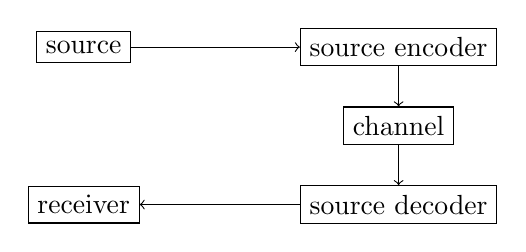
\begin{tikzpicture}
        \tikzstyle{blk} = [draw, black]
        
        \node[draw] (source) at (0, 0) {source};
        \node[draw] (encoder) at (4, 0) {source encoder};
        \node[draw] (channel) at (4, -1) {channel};
        \node[draw] (decoder) at (4, -2) {source decoder};
        \node[draw] (receiver) at (0, -2) {receiver};
        
        \path[blk, ->] (source) to (encoder);
        \path[blk, ->] (encoder) to (channel);
        \path[blk, ->] (channel) to (decoder);
        \path[blk, ->] (decoder) to (receiver);
    \end{tikzpicture}
    \caption{source coding is used to send data across a channel}
    \label{fig:datapath}
\end{figure}

\begin{example} \label{ex:source}
    Consider the source encoding of four trees, \textit{ash}, \textit{birch}, \textit{cherry}, \textit{maple}, as follows:
    \[
        \text{ash} \to 00, \hspace{10pt}\text{birch} \to 01, \hspace{10pt} \text{cherry} \to 10, \hspace{10pt} \text{maple} \to 11.
    \]
    The 2 bit encoding is much smaller and more suitable for sending over a channel than the original words.
\end{example}

Since source coding is performed on data with the intention of sending the data over a channel, there is a chance that noise in the channel might change the source coding and cause the wrong information to be sent. Noise can be thought of as interference. For example, noise can sometimes be heard on radio transmissions as static. So, using the source coding scheme from Example \ref{ex:source}, if we sent the message `\textit{ash}, \textit{birch}, \textit{cherry}, \textit{maple}' which would be sent as the binary encoding `$00011011$' channel noise might cause a bit to switch and the message to come out of the channel as `$01011011$' which would be the message `\textit{birch}, \textit{birch}, \textit{cherry}, \textit{maple}.' This is an example, depicted in figure \ref{fig:pathexample}, of an error being introduced to a coded message. This is where channel coding and error-correcting codes become useful.

\begin{figure}
\centering
    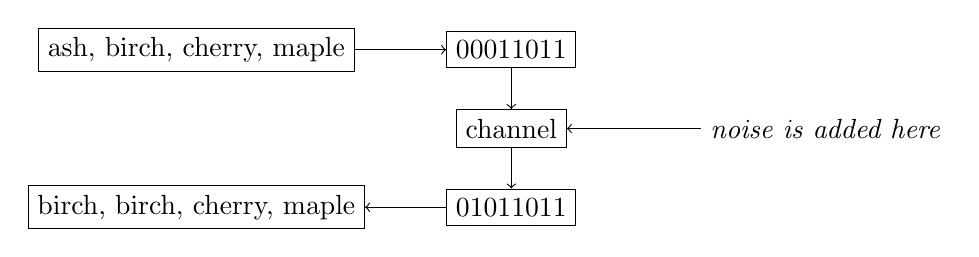
\begin{tikzpicture}
        \tikzstyle{blk} = [draw, black]
        
        \node[draw] (source) at (0, 0) {ash, birch, cherry, maple};
        \node[draw] (encoder) at (4, 0) {00011011};
        \node[draw] (channel) at (4, -1) {channel};
        \node[] (noise) at (8, -1) {\textit{noise is added here}};
        \node[draw] (decoder) at (4, -2) {01011011};
        \node[draw] (receiver) at (0, -2) {birch, birch, cherry, maple};
        
        \path[blk, ->] (source) to (encoder);
        \path[blk, ->] (encoder) to (channel);
        \path[blk, ->] (noise) to (channel);
        \path[blk, ->] (channel) to (decoder);
        \path[blk, ->] (decoder) to (receiver);
    \end{tikzpicture}
    \caption{a coding error has occurred}
    \label{fig:pathexample}
\end{figure}

\section{Error-Correcting Codes}

\textit{Channel coding} makes use of error-correcting codes. The simplest examples of which are repetition codes and single-parity-check codes. We can use $k$ to represent the block length of a source coded message, $r$ to represent the number of digits added by the channel encoding. The length of a channel block after the channel encoding is $n = k + r$.

There are $2^n$ possible words of length $n$ that can be received. The set of all $2^k$ words of length $n$ that correspond to the $2^k$ possible source code blocks that can be encoded is called the \textit{code} and these words are each a \textit{codeword}.

\begin{figure}
    \centering
    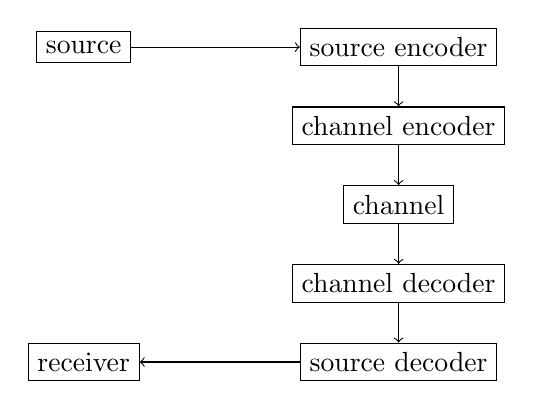
\begin{tikzpicture}
        \tikzstyle{blk} = [draw, black]
        
        \node[draw] (source) at (0, 0) {source};
        \node[draw] (source encoder) at (4, 0) {source encoder};
        \node[draw] (channel encoder) at (4, -1) {channel encoder};
        \node[draw] (channel) at (4, -2) {channel};
        \node[draw] (channel decoder) at (4, -3) {channel decoder};
        \node[draw] (source decoder) at (4, -4) {source decoder};
        \node[draw] (receiver) at (0, -4) {receiver};
        
        \path[blk, ->] (source) to (source encoder);
        \path[blk, ->] (source encoder) to (channel encoder);
        \path[blk, ->] (channel encoder) to (channel);
        \path[blk, ->] (channel) to (channel decoder);
        \path[blk, ->] (channel decoder) to (source decoder);
        \path[blk, ->] (source decoder) to (receiver);
    \end{tikzpicture}
    \caption{channel coding is used to account for channel noise}
    \label{fig:channelcodingpath}
\end{figure}

A \textit{repetition code} just repeats each binary digit multiple times and the decoder simply uses the digit repeated the most times to interpret the original digit in the source code. If $r$ is odd then there could be an equal number of zeros and ones in a block, this results in the decoder returning a decoding failure for that block. For a repetition code, $k = 1$, $r$ can be whatever the sender decides, and $n = r + k = r + 1$.

\begin{example} \label{ex:repeat}
    Consider encoding the message `\textit{ash}, \textit{birch}, \textit{cherry}, \textit{maple}' using the source codes from Example \ref{ex:source} with a repetition code where $r = 4$. The channel coding would be
    \[
        00011011 \to 00000\ 00000\ 00000\ 11111\ 11111\ 00000\ 11111\ 11111.
    \]
    The decoder chooses the digit repeated the most times from each sequence of $5$ bits corresponding to a digit of the source code. As long as each of these sequences has less than $\left\lceil\frac{1}{2}(r + 1)\right\rceil = 3$ errors introduced from channel noise, the correct message is decoded as depicted in figure \ref{fig:repititionpathexample}.
    
\end{example}

\begin{figure}
    \centering
    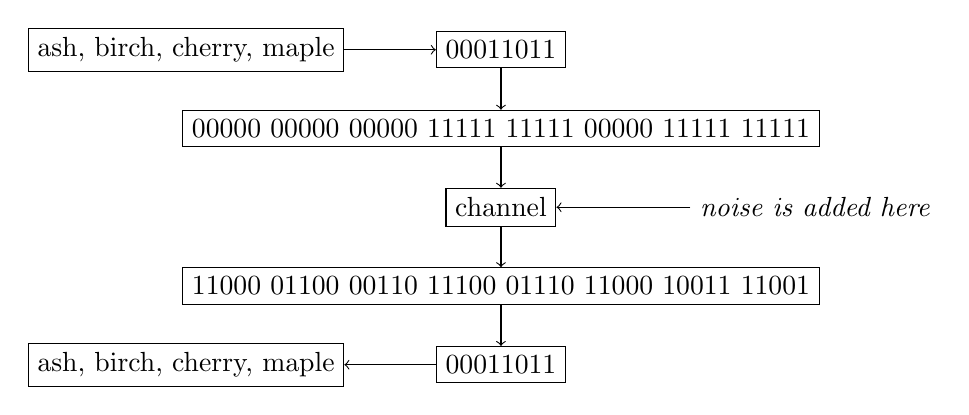
\begin{tikzpicture}
        \tikzstyle{blk} = [draw, black]
        
        \node[draw] (source) at (0, 0) {ash, birch, cherry, maple};
        \node[draw] (source encoder) at (4, 0) {00011011};
        \node[draw] (channel encoder) at (4, -1) {00000 00000 00000 11111 11111 00000 11111 11111};
        \node[draw] (channel) at (4, -2) {channel};
        \node[draw] (channel decoder) at (4, -3) {11000 01100 00110 11100 01110 11000 10011 11001};
        \node[draw] (source decoder) at (4, -4) {00011011};
        \node[draw] (receiver) at (0, -4) {ash, birch, cherry, maple};
        \node[] (noise) at (8, -2) {\textit{noise is added here}};
        
        \path[blk, ->] (source) to (source encoder);
        \path[blk, ->] (source encoder) to (channel encoder);
        \path[blk, ->] (channel encoder) to (channel);
        \path[blk, ->] (channel) to (channel decoder);
        \path[blk, ->] (channel decoder) to (source decoder);
        \path[blk, ->] (source decoder) to (receiver);
        \path[blk, ->] (noise) to (channel);
    \end{tikzpicture}
    \caption{even with the introduction of two errors per block, the repetition code returns the correct message}
    \label{fig:repititionpathexample}
\end{figure}

A \textit{single-parity-check code} takes the sum of the binary digits of a source code message modulo $2$ (the binary sum), and concatenates this digit to the end of the source-coded message block. For a single-parity-check-code, $k$ can be any length we choose up to the length of the entire message, $r = 1$, and $n = k + r = k + 1$.

\begin{example} \label{ex:single}
    Consider encoding the same message from Example \ref{ex:repeat} using a single-parity-check-code with $k$ equal to the length of the message. Since
    \[
        0 + 0 + 0 + 1 + 1 + 0 + 1 + 1 \equiv 0 \pmod{2},
    \]
    the channel coding would be
    \[
        00011011 \to 000110110.
    \]
    If the binary sum of the first $n - 1$ digits of the received message is equal to the last digit of the received message then the decoder decodes the message, otherwise it assumes an error was introduced and returns a decoding failure. If noise adds an even number of errors to the first $n - 1$ digits, or an odd number of errors and the last digit changes, then the message is decoded incorrectly.
\end{example}

Repetition codes have extremely high error detection capability because they can repeat digits as many times as the sender wants. They also, however, have an extremely low information rate because each block only sends a single digit of the source code. Single-parity-check codes are the opposite of this with an extremely high information rate but extremely low error detection capability. All the error-correcting codes used for encryption will fall somewhere between these two extremes. Typically, encryption makes use a of linear codes which are a type of error-correcting code.

\section{Linear Codes}\label{linearcodessection}

For any code containing several message digits and several check digits, the check digits must be a function of the message digits. The function for single-parity-check codes, for example, is the binary sum of the message digits. As mentioned before, a \textit{linear code} is an error-correcting code for which any linear combination of codewords is a codeword. We will construct a basic example with $k = 3$, $r = 3$ and $n = k + r = 6$.

\begin{example}\label{ex:simlin}
    Let $C_1$, $C_2$, and $C_3$ be the message digits of our linear code. Choose $C_4$, $C_5$, and $C_6$ as check digits that satisfy
    \[
        \left[\begin{array}{c}
            C_4\\
            C_5\\
            C_6
        \end{array}\right] = 
        \left[\begin{array}{ccc}
            1 & 1 & 0\\
            1 & 0 & 1\\
            0 & 1 & 1
        \end{array}\right]
        \left[\begin{array}{c}
            C_1\\
            C_2\\
            C_3
        \end{array}\right].
    \]
    Every codeword $\mathbf{C}$ consists of a linear combination of the digits $C_1, C_2, C_3, C_4, C_5, C_6$ and must satisfy
    \[
        \mathscr{H}\textbf{C}^t = \textbf{0}
    \]
    where $\textbf{C}^t$ denotes the column vector which is the transpose of the row vector
    \[
        \textbf{C} = [C_1, C_2, C_3, C_4, C_5, C_6],
    \]
    $\textbf{0}$ is the zero vector in $\mathbb{F}_2^3$, and $\mathscr{H}$ is the \textit{parity-check matrix}
    \[
        \mathscr{H} = 
        \left[\begin{array}{cccccc}
            1 & 1 & 0 & 1 & 0 & 0\\
            1 & 0 & 1 & 0 & 1 & 0\\
            0 & 1 & 1 & 0 & 0 & 1\\
        \end{array}\right].
    \]
    Once a codeword is sent across a noisy channel, any noise received can be written as the word (the terms word and vector are interchangeable here) $\textbf{E} = [E_1, E_2, E_3, E_4, E_5, E_6]$ where
    \[
        E_i = \begin{cases}
            0 & \text{if the channel does not change the $i$th digit}\\
            1 & \text{if the channel changes the $i$th digit}
        \end{cases}.
    \]
    The received word is $\textbf{R} = [R_1, R_2, R_3, R_4, R_5, R_6]$ where $R_i = C_i + E_i$ and so $\textbf{R} = \textbf{C} + \textbf{E}$. Upon receiving a word, the decoder would first compute the \textit{syndrome}, denoted $\textbf{s}$, of the word where
    \[
        \textbf{s}^t = \mathscr{H}\textbf{R}^t.
    \]
    Since this is a linear code, the set of codewords form a group under addition. For this reason, a linear code can also be referred to as \textit{group code}. Any set of words which have the same syndrome form a \textit{coset} of this group. Each word has \textit{weight} equal to sum of its $n = k + r$ binary digits. The word within each coset with least weight is chosen to be the \textit{coset leader}. Once the decoder has computed the syndrome of a received word, it finds the leader of the coset with this syndrome, then subtracts the coset leader of this coset from the received word which provides the codeword that had the highest probability of being transmitted, given that errors are assumed to be relatively infrequent.
\end{example}
    
\begin{definition}\label{lineardef}
    A code is said to be a \textit{linear} code or \textit{group} code iff its codewords are the set of vectors $\textbf{C}$ which satisfy an equation $\mathscr{H}\textbf{C}^t = \textbf{0}$. The matrix $\mathscr{H}$ is called the \textit{parity-check matrix}. The \textit{syndrome} $\textbf{s}$ of any word $\textbf{R}$ is defined by the equation $\textbf{s}^t = \mathscr{H}\textbf{R}^t$. A \textit{coset} consists of all words having a given syndrome. The \textit{weight} of any word is the number of ones among its $n$ digits. Within each coset, a word having the least weight is chosen as \textit{coset leader}.
\end{definition}

We often denote such a code $C$, where $C$ represents the set of codewords. This allows for a more concise definition.

\begin{definition}
    A \textit{linear code} $C$ of length $n$ over $\mathbb{F}_q^n$ is a subspace of $\mathbb{F}_q^n$.
\end{definition}

\begin{theorem} (\cite{berlekamp})
    If $\textbf{R}$ is the received word, the set of possible error words is the coset containing $\textbf{R}$. A most probable error word is the leader of the coset containing $\textbf{R}$. A linear code may be decoded as follows. Compute the syndrome, find the leader of the coset having this syndrome, and subtract this coset leader from the received word to find a most likely transmitted codeword.
\end{theorem}

Repetition codes and single-parity-check codes form the most trivial examples of linear codes. For the repetition code given in Example \ref{ex:repeat},
\[
    \mathscr{H} = \left[\begin{array}{ccccc}
        1 & 1 & 0 & 0 & 0\\
        1 & 0 & 1 & 0 & 0\\
        1 & 0 & 0 & 1 & 0\\
        1 & 0 & 0 & 0 & 1\\
    \end{array}\right]
\]
and for the single-parity-check code given in Example \ref{ex:single},
\[
    \mathscr{H} = \left[\begin{array}{ccccccccc}
        1 & 1 & 1 & 1 & 1 & 1 & 1 & 1 & 1
    \end{array}\right].
\]
The first error-correcting code, which is also a linear code, was the Hamming code.

\subsection{Hamming Codes}

We can see that $\textbf{s}^t = \mathscr{H}\textbf{E}^t$ since
\begin{align}
    \textbf{s}^t = \mathscr{H}\textbf{R}^t &\implies \textbf{s}^t = \mathscr{H}\left(\textbf{C}^t + \textbf{E}^t\right)\\
    &\implies \textbf{s}^t = \textbf{0} + \mathscr{H}\textbf{E}^t\\
    &\implies \textbf{s}^t = \mathscr{H}\textbf{E}^t
\end{align}
where the $\textbf{0}$ on line (2.2) is the zero vector in $\mathbb{F}_2^n$. Thus, the syndrome is the sum of the columns of $\mathscr{H}$ where any channel errors occur. Therefore, all columns of $\mathscr{H}$ must be distinct and nonzero in order for a linear code to be capable of correcting all patterns of a single error. Otherwise multiple single error patterns will lie in the same coset and only one will be chosen as coset leader which will lead to the other single error patterns being incorrectly decoded.

\begin{theorem} (\cite{berlekamp})
    A linear binary code is capable of correcting all patterns of not more than one channel error iff all columns of its $\mathscr{H}$ matrix are distinct and nonzero.
\end{theorem}

Since the number of check digits, $r$, is equal to the row rank of $\mathscr{H}$, the longest block length possible for a single-error-correcting code having at most $r$ check digits is the maximum number of distinct nonzero columns which can occur in a binary matrix having at most $r$ rows. Thus, the longest block length possible for a single-error-correcting code having at most $r$ check digits is $2^r - 1$. In this case, the columns of $\mathscr{H}$ are the $2^r - 1$ nonzero binary $r$-tuples, arranged in any order. A linear code defined by such a $\mathscr{H}$ is called a \textit{Hamming code}.

There exists a binary Hamming code for any $r$ containing $r$ check digits with block length $n = 2^r - 1$ and $k = n - r = 2^r - 1 - r$ information digits.

\begin{example}\label{ex:hamming}
    If we wish to modify Example $\ref{ex:simlin}$ to make it a Hamming code, we need to concatenate the column $\textbf{1}^3$ to $\mathscr{H}$. Since we can arrange the columns in any order, arranging the columns lexicographically provides
    \[
        \mathscr{H} = 
        \left[\begin{array}{ccccccc}
            0 & 0 & 0 & 1 & 1 & 1 & 1\\
            0 & 1 & 1 & 0 & 0 & 1 & 1\\
            1 & 0 & 1 & 0 & 1 & 0 & 1\\
        \end{array}\right].
    \]
    This code allows us to have $k = 4$ information digits with the same number of check digits, which is $r = 3$, as Example \ref{ex:simlin}.
\end{example}

If we wish to modify a Hamming code so that we can not only correct channel-error patterns of weight $\leq 1$ and detect channel-error patterns of weight $2$, but also detect channel-error patterns of weight 3, we need to annex an additional overall parity check to the Hamming code. The resulting code will have block length $n = 2^m$, $r = m + 1$ check digits, and $k = 2^m - 1 - m$ information digits. Such a code is called an \textit{extended} Hamming code.

\begin{example}\label{ex:extendedhamming}
    Creating an extended Hamming code from Example \ref{ex:hamming} yields
    \[
        \mathscr{H} = 
        \left[\begin{array}{cccccccc}
            1 & 1 & 1 & 1 & 1 & 1 & 1 & 1\\
            0 & 0 & 0 & 0 & 1 & 1 & 1 & 1\\
            0 & 0 & 1 & 1 & 0 & 0 & 1 & 1\\
            0 & 1 & 0 & 1 & 0 & 1 & 0 & 1\\
        \end{array}\right]
    \]
    which is capable of detecting an error pattern of weight up to 3 and, in this case, return a decoding failure rather than an incorrect message.
\end{example}

Hamming codes were developed in 1950 and are unable to correct any pattern of two or more errors. It took until the development of Bose-Chaudhuri-Hocquenghem codes (BCH codes) in 1960 to be able to correct more than one error.

\subsection{BCH Codes}

We introduce BCH codes by constructing a BCH code capable of correcting two or fewer errors. The first step is to construct a Hamming code so that we may correct a single error. Next, we need to add additional rows to $\mathscr{H}$ in order to correct a second error. We can create a second Hamming code in these rows but it needs to be different enough so that our code can tell the difference between our first and second error. However, in order to be a Hamming code, it will need to be a permutation of the original Hamming code. So we need to use a function $f(\xi)$ mapping nonzero the binary $r$-tuples representing the rows of the first Hamming code to nonzero binary $r$-tuples which also satisfies these properties.

We can interpret binary vectors in $\mathbb{F}_2^r$ as binary polynomials of degree $r - 1$. If we label our error positions as $\beta_1$ and $\beta_2$, our first Hamming code will give us $\zeta_1 = \beta_1 + \beta_2$. Our second Hamming code will correspond to $\zeta_2 = f(\beta_1) + f(\beta_2)$. In order to solve for $\beta_1$ and $\beta_2$, we can not have the equations for $\zeta_1$ and $\zeta_2$ be dependent.

If we interpret $\xi$ as a binary polynomial of degree $r - 1$ and define $f:\mathbb{F}_2^r \to \mathbb{F}_2^r$ to be
\[
    f(\xi) = \xi^3 \mod (2, M(x))
\]
where $M(x)$ is a binary \textit{irreducible polynomial} of degree $r$, then we get what we wanted. In this case, the decoder's equations will be
\[
    \beta_1 + \beta_2 = \zeta_1 \hspace{10pt} \text{and} \hspace{10pt} \beta_1^3 + \beta_2^3 = \zeta_2
\]
and, assuming that $\zeta_1 \neq 0$, both $\beta_1$ and $\beta_2$ will end up satisfying the quadratic equation
\[
    \beta^2 + \zeta_1\beta + \left(\zeta_1^2 + \frac{\zeta_2}{\zeta_1}\right) = 0.
\]
So the roots of the above quadratic equation will correspond to the two error locations in the received word. If $\zeta_1 = 0$ then there are no errors and the decoder has received a codeword. If there is only one error then $\beta_1$ provides the error's location.

\begin{example}\label{ex:2BCH}
    We will use the the same type of Hamming code as Example \ref{ex:hamming} for our starting point, only we will be looking at the version when $r = 4$ and $n = 15$. To be able to correct up to two errors we can use $f(\xi) = \xi^3$ as described above to get
    \[
        \mathscr{H} = 
        \left[\begin{array}{cccccccccc}
            0 & 0 & 0 & 0 & 0 & 0 & 0 & \cdots & 1 & 1\\
            0 & 0 & 0 & 1 & 1 & 1 & 1 & \cdots & 1 & 1\\
            0 & 1 & 1 & 0 & 0 & 1 & 1 & \cdots & 1 & 1\\
            1 & 0 & 1 & 0 & 1 & 0 & 1 & \cdots & 0 & 1\\
            f_1(\xi_1) & f_1(\xi_2) & f_1(\xi_3) & f_1(\xi_4) &f_1(\xi_5) & f_1(\xi_6) & f_1(\xi_7) & \cdots & f_1(\xi_{14}) & f_1(\xi_{15})\\
            f_2(\xi_1) & f_2(\xi_2) & f_2(\xi_3) & f_2(\xi_4) &f_2(\xi_5) & f_2(\xi_6) & f_2(\xi_7) & \cdots & f_2(\xi_{14}) & f_2(\xi_{15})\\
            f_3(\xi_1) & f_3(\xi_2) & f_3(\xi_3) & f_3(\xi_4) &f_3(\xi_5) & f_3(\xi_6) & f_3(\xi_7) & \cdots & f_3(\xi_{14}) & f_3(\xi_{15})\\
            f_4(\xi_1) & f_4(\xi_2) & f_4(\xi_3) & f_4(\xi_4) &f_4(\xi_5) & f_4(\xi_6) & f_4(\xi_7) & \cdots & f_4(\xi_{14}) & f_4(\xi_{15})\\
        \end{array}\right]
    \]
    where $\xi_i$ represents the $i$th row of the Hamming code making up the first three rows of $\mathscr{H}$ and $f_j$ represents the $j$th digit of the output of $f(\xi)$. In this case, we need $M(x)$ to be an irreducible polynomial of degree $r = 4$. So we can let $M(x) = x^4 + x^3 + x^2 + x + 1$. Thus, the parity-check matrix
    \[
        \mathscr{H} = 
        \left[\begin{array}{ccccccccccccccc}
            0 & 0 & 0 & 0 & 0 & 0 & 0 & 1 & 1 & 1 & 1 & 1 & 1 & 1 & 1\\
            0 & 0 & 0 & 1 & 1 & 1 & 1 & 0 & 0 & 0 & 0 & 1 & 1 & 1 & 1\\
            0 & 1 & 1 & 0 & 0 & 1 & 1 & 0 & 0 & 1 & 1 & 0 & 0 & 1 & 1\\
            1 & 0 & 1 & 0 & 1 & 0 & 1 & 0 & 1 & 0 & 1 & 0 & 1 & 0 & 1\\
            0 & 1 & 1 & 0 & 1 & 0 & 1 & 1 & 0 & 0 & 1 & 0 & 0 & 0 & 0\\
            0 & 0 & 1 & 0 & 0 & 1 & 0 & 1 & 1 & 0 & 1 & 0 & 0 & 0 & 1\\
            0 & 0 & 1 & 1 & 0 & 0 & 0 & 1 & 0 & 1 & 1 & 0 & 0 & 1 & 0\\
            1 & 0 & 1 & 0 & 0 & 0 & 0 & 1 & 0 & 0 & 1 & 1 & 1 & 0 & 0\\
        \end{array}\right]
    \]
    provides BCH code capable of correcting up to two errors with the same set of codewords as Example \ref{ex:hamming}. \color{red}(the bottom half of this matrix is wrong and needs to be fixed) \color{black} While building to BCH codes has provided us a convenient way to work our way up to linear error-correcting codes capable of correcting multiple errors, the actual type of codes most commonly used in modern implementable cryptographic schemes are Goppa codes.
\end{example}

\subsection{Goppa Codes}

Goppa codes, also sometimes referred to as algebraic geometric codes (AG-codes), are linear codes which utilize algebraic curves over finite fields \cite{GoppaCodes}.

\begin{theorem}[Riemann-Roch Theorem]\label{rrtheorem}(\cite{riemann-roch})
    Let $C$ be a non-singular projective plane curve of genus $g$ defined over $\mathbb{F}_q$ and let $D$ be a divisor on $C$. Then $\dim [L(D)] \geq \deg (D + 1 - g)$ Further, if $\deg(D) > 2g - 2$, then
    \[
        \dim[L(D)] = \deg(D + 1 - g).
    \]
\end{theorem}

\begin{definition}
    Let $\mathbf{X}$ be a smooth projection curve over a finite field $\mathbb{F}_q$. Let
    \[
        \mathcal{P} = \{P_1, P_2, \dots, P_n\} \subset \mathbf{X}(\mathbb{F}_q)
    \] be a set of distinct $\mathbb{F}_q$-rational points on $\mathbf{X}$. Let $G$ be a divisor of $\mathbf{X}$ with a support consisting of only rational points with
    \[
        \mathcal{P} \cap \supp(G) = \varnothing.
    \]
    By theorem \ref{rrtheorem}, there exists a unique finite-dimensional vector space, $L(G)$, with respect to $G$. Let $D = P_1 + P_2 + \cdots + P_n$ be a divisor on \color{red} something\color{black}. A \textit{Goppa code}, denoted $C(D, G)$, is defined by
    \[
        C(D, G) = \{(f(P-1), f(P_2), \dots, f(P_n)) \mid f \in L(G)\} \subset \mathbb{F}_q^n.
    \]
\end{definition}

While this definition describes the class of general Goppa codes, we are only concerned with binary Goppa codes specifically.


\subsubsection{Binary Goppa Codes}

Binary Goppa codes belong to the class of general Goppa codes. The binary structure of these codes provides some mathematical advantages over non-binary variants. Binary also provides us a better integration with computer application. Binary Goppa codes are the codes used in the McEliece cryptosystem, as well as other cryptosystems similar to the McEliece cryptosystem.

Let $g(x)$ be a polynomial of degree $t$ over a finite field, $\mathbb{F}_{2^m}$ for some fixed $m$, with no repeated roots. Let $L_1, L_2, \dots, L_n$ be a sequence of $n$ distinct elements in $\mathbb{F}_{2^m}$ which are not roots of $g$. The set of codewords $\mathbf{C} = (C_1, C_2, \dots, C_n) \in \mathbb{F}_2^n$, form a subspace of $\{0, 1\}^n$. The \textit{Goppa code} $\Gamma(L, g)$ is defined as
\[
    \Gamma(L, g) = \left\{\mathbf{C} \in \{0, 1\}^n \bigg| \sum_{i = 1}^n \frac{C_i}{x - L_i} \equiv 0 \pmod{g(x)}\right\}.
\]
The polynomial $g(x)$ is called the \textit{Goppa polynomial}, and when $g(x)$ is irreducible, $\Gamma(L, g)$ is called an \textit{irreducible} Goppa code.

Note that some properties of $\Gamma(g, L)$ are that $\dim(\Gamma(g, L)) \geq n - mt$ and the minimum distance is $2t + 1$. This means the code can encode messages of at least length $n - mt$ when using codewords of size $n$, with a capability of correcting at least
\[
    \left\lfloor\frac{(2t + 1) - 1}{2}\right\rfloor
\]
errors. The parity check matrix for such a code is
\[
    \mathscr{H} = \left[\begin{array}{ccccc}
        1 & 1 & 1 & \cdots & 1\\
        L_1^1 & L_2^1 & L_3^1 & \cdots & L_n^1\\
        L_1^2 & L_2^2 & L_3^2 & \cdots & L_n^2\\
        \vdots & \vdots & \vdots & \ddots & \vdots\\
        L_1^{t - 1} & L_2^{t - 1} & L_3^{t - 1} & \cdots & L_n^{t - 1}
    \end{array}\right]\left[\begin{array}{ccccc}
        \frac{1}{g(L_1)} &  &  &  & \\
         & \frac{1}{g(L_2)} &  &  & \\
         &  & \frac{1}{g(L_2)} &  & \\
         &  &  & \ddots & \\
         &  &  &  & \frac{1}{g(L_n)}\\
    \end{array}\right]
\]
which is seen here written as a product of a Vandermonde matrix and a diagonal matrix. When used in application $\mathscr{H}$ will be converted to binary via a trace construction. This converts the above $t \times n$ matrix over $\mathbb{F}_{2^m}$ into an $mt \times n$ binary matrix. The binary matrix consists of the polynomial coefficients from $\mathbb{F}_{2^m}$ written as the entries of $m$ successive rows. This is similar to what was done in the previous BCH codes section. Using such binomial entries allows for easier computer application of any codes.

\section{McEliece Cryptosystem}

The McEliece cryptosystem, named after its creator, was developed in 1978. The cryptosystem relies off of the hardness of decoding a general linear code, which is known to be NP-hard. Thus far, the McEliece scheme, along with its use of Goppa codes, has resisted cryptanalysis and appears to remain secure even in age of quantum computing because of its immunity to attacks using Shor's algorithm. The scheme does, however, require its key size to be increased by a factor of four to remain secure for quantum computing \cite{10.1007/978-3-642-12929-2_6}.

There exists many variants of the McEliece scheme, which were motivated by a desire to reduce the size of the scheme's keys. The variants attempt to do this by introducing more structure into the code.  Most of these variants, however, have been proven to be less secure \cite{Overbeck2009}.

The cryptosystem utilizes three algorithms, two probabilistic and one deterministic. 

\subsection{McEliece Algorithms}\label{subsec:mceliecealgo}

The McEliece cryptosystem was the first cryptographic scheme to utilize randomization, which it does in the probabilistic algorithms. One of the probabilistic algorithms produces a public and private key, the other encrypts the data. The deterministic algorithm is used to decrypt the data.

Note that the McEliece cryptosystem has a faster encryption and decryption than RSA. The reason RSA is currently preferred is because of the McEliece cryptosystem's large key sizes. While it was originally thought that the McEliece cryptosystem could not produce a digital signature, a variation was created, known as the Niederreiter scheme, which is capable of constructing a signature scheme \cite{10.1007/3-540-45682-1_10}. This variation will be discussed in the next section.

Utilizing the convention established by Rivest, Shamir, and Adleman in 1978, we will suppose that Alice and Bob are two users of a public-key cryptosystem \cite{10.1145/359340.359342}. Alice and Bob share a set of common public security parameters which we will denote $k$, $n$, and $t$.

\begin{definition}
    If $C$ is a linear code that, as a vector space over the field $\mathbb{F}^n$, has dimension $k$, then we say that $C$ is an $(n, k)$ \textit{linear code} over $\mathbb{F}^n$, or an $(n, k)$-code, for short.
\end{definition}

\subsubsection{Key Generation Algorithm}

The key generation algorithm (shown here for Alice) is as follows \cite{1978DSNPR..44..114M}:

\begin{enumerate}
    \item Alice selects a binary $(n, k)$-code $C$, capable of correcting up to $t$ errors; in practice, the cryptosystem uses Goppa codes. The chosen $n$ and $k$ values correspond with the linear code as described in section \ref{linearcodessection} \color{red}(need to verify this)\color{black}. The choice of code will give rise to an efficient decoding algorithm, which we can denote $A$. Let $G$ be a generator matrix for $C$ \color{red}(need to define generator matrices somewhere before this)\color{black}, typically there is a natural choice for $G$. The generator matrix $G$ is kept secret since it can be used to find $A$.
    
    \item Alice selects a randomly generated $n \times n$ binary non-singular matrix, which we denote $S$.
    
    \item Alice selects a randomly generated $n \times n$ permutation matrix, which we denote $P$.
    
    \item Alice computes $\hat G = SGP$, a $k \times n$ matrix called the public generator matrix.
\end{enumerate}
Alice's private key is $(S, P, A)$ and her public key is $\left(\hat G, t\right)$.

\subsubsection{Message Encryption Algorithm}

Now that Alice has the public key $\left(\hat G, t\right)$, we suppose that Bob wants to send a message, denoted $m$, to Alice. The message encryption algorithm is as follows \cite{1978DSNPR..44..114M}:

\begin{enumerate}
    \item Bob encodes $m$ as a binary string of length $k$.
    
    \item Bob computes the vector $c' = m \hat G$.
    
    \item Bob generates a random binary vector, labelled $z$, of length $n$ with exactly $t$ ones.
    
    \item Bob computes the ciphertext $c = c' + z$.
\end{enumerate}

\subsubsection{Message Decryption Algorithm}

Now that Bob has computed the ciphertext, we suppose Alice receives the ciphertext $c$. The message decryption algorithm is as follows \cite{1978DSNPR..44..114M}:

\begin{enumerate}
    \item Alice computes $P^{-1}$, the inverse of $P$.
    
    \item Alice computes $\hat c = cP^{-1}$.
    
    \item Alice uses $A$ to decode $\hat c$, we denote the decoded $\hat c$ as $\hat m$.
    
    \item Alice computes $m = \hat m S^{-1}$.
\end{enumerate}

\section{Niederreiter Cryptosystem}

The Niederreiter cryptosystem, named after its creator, is a variation of the McEliece cryptosystem which was developed in 1986. The encryption of the Niederreiter scheme is faster than the McEliece scheme and the scheme allows for construction of a digital signature scheme, which was not possible with the McEliece scheme.

\subsection{Niederreiter Algorithms}

The Niederreiter algorithms provide an equivalent level of security to those of the McEliece. There are some key differences.

\subsubsection{Key Generation}

The key generation algorithm (shown here for Alice) is as follows \cite{80003180051}:

\begin{enumerate}
    \item Alice selects a binary $(n, k)$ code, labelled $G$, capable of correcting $t$ errors. In this case the code should be a Goppa code because a case of the Niederreiter scheme was broken when not using a Goppa code \cite{SIDELNIKOVSHESTAKOV+1992+439+444}. The code once again gives rise to an efficient decoding algorithm, which we can denote $A$.
    
    \item Alice generates a $(n - k) \times n$ parity check matrix, denoted $H$, for $G$.
    
    \item Alice selects a randomly generated $(n - k) \times (n - k)$ binary non-singular matrix, which we denote $S$.
    
    \item Alice selects a randomly generated $n \times n$ permutation matrix, which we denote $P$.
    
    \item Alice computes the matrix $H^{\mathrm{pub}} = SHP$, a $(n - k) \times n$ matrix.
\end{enumerate}
Alice's private key is $(S, H, P)$ and her public key is $\left(H^{\mathrm{pub}}, t\right)$.

\subsubsection{Message Encryption}

Now that Alice has the public key $\left(H^{\mathrm{pub}}, t\right)$, we suppose that Bob wants to send a message, denoted $m$, to Alice. The message encryption algorithm is as follows \cite{80003180051}:

\begin{enumerate}
    \item Bob encodes $m$ as a binary string, labelled $e$, of length $n$ with exactly $t$ ones.
    
    \item Bob computes the ciphertext $c = H^{\mathrm{pub}}e^{\mathrm{T}}$ (we use $^\mathrm{T}$ to represent the transpose since $t$ is already being used to represent the number of errors $G$ is capable of correcting).
\end{enumerate}

\subsubsection{Message Decryption}

Now that Bob has computed the ciphertext, we suppose Alice receives the ciphertext $c$. The message decryption algorithm is as follows \cite{80003180051}:

\begin{enumerate}
    \item Alice computes $S^{-1}c = S^{-1}H^{\mathrm{pub}}e^\mathrm{T} = HPe^\mathrm{T}$.
    
    \item Alice uses $A$ to to recover $Pe^{\mathrm{T}}$.
    
    \item Alice computes $P^{-1}Pe^{\mathrm{T}} = e^\mathrm{T}$. This provides $e$ which can be decoded to obtain $m$.
\end{enumerate}